\documentclass{beamer}
%\usetheme[footline=infoline,headline=secheader]{UPB}
%\usetheme[footline=infoline,headline=structure]{UPB}
%\usetheme[headline=secheader]{UPB}
%\usetheme[headline=structure]{UPB}
%\usetheme[footline=infoline]{UPB}
%\usetheme{UPB} % defaults are footline=empty,headline=empty
%\usetheme{Antibes}
\usetheme{upb}
\usepackage[utf8]{inputenc}
\usepackage{hyperref}
\author[C.Robbert, P. Stilow]{Christoph Robbert, Peter Stilow}
\institute[Uni Paderborn]{Universität Paderborn}
\title[WLAN Security]{WLAN Security}
\begin{document}
\begin{frame}
\maketitle
\end{frame}

\section{Übersicht}
\begin{frame}
\frametitle{WLAN Grundlagen}
\begin{itemize}
	\item Direkte Kommunikation (AdHoc)
	\item Access Point
	\item Frequenzen zwischen 2,4 und 5,2 GHz
	\item Strahlt in alle Richtungen
\end{itemize}
Probleme:
\begin{itemize}
	\item Kann in einem gewissen Bereich empfangen werden ($\rightarrow$ abhören / Daten einspeisen)
	\item Kollisionen mit anderen WLANs (oder Störsender)
	\item Auto-Connection zu offenen (gefälschten) Access Points
	\item[$\rightarrow$] Offen (+ VPN o.ä.) oder Verschlüsselung Notwendig
\end{itemize}
\end{frame}

\begin{frame}
\frametitle{WLAN Sicherheit}
\begin{itemize}
	\item WEP (802.11)
	\item WPA/WPA2 (802.11i)
	\item WPS
\end{itemize}
\end{frame}

\section{WEP}
\begin{frame}
\frametitle{WEP - Wired Equivalent Privacy}
\begin{figure}
	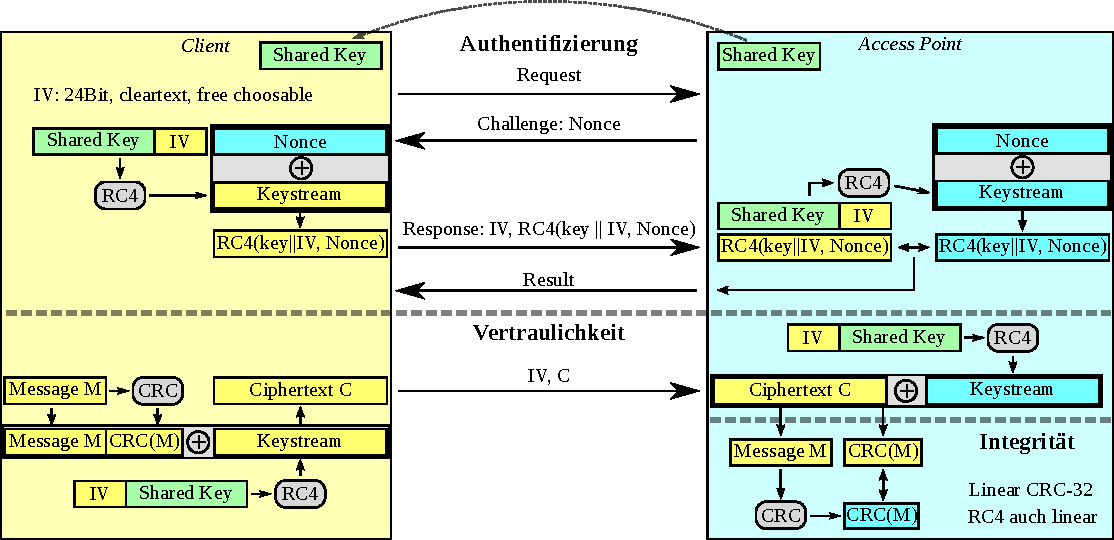
\includegraphics[width=1.0\linewidth]{figures/WEP_complete.pdf}
\end{figure}
\end{frame}


\section{Attacken gegen WEP}
\begin{frame}
\frametitle{Testing the beamer style}
\begin{itemize}
	\item test
	\item test2
\end{itemize}

\end{frame}


\section{WPA/WPA2(802.11i)}
\begin{frame}
\begin{itemize}
	\item Keines der Schutzziele von WEP (Authentizität, Vertraulichkeit, Integrität) wird erfüllt
	\item[$\Rightarrow$] Entwicklung von 802.11i (WPA/WPA2)
\end{itemize}
\begin{block}{802.11i}
\begin{itemize}
	\item Schlüsselverwaltung:
	\begin{itemize}
		\item Personal/ Pre-Shared Key (PSK)
		\item Enterprise (802.1X)
	\end{itemize}
	\item Sicherheitsprotokolle:
	\begin{itemize}
		\item TKIP(WPA, optional WPA2)
		\item AES-CCMP(optional WPA, WPA2)
	\end{itemize}
\end{itemize}
\end{block}
\end{frame}

\begin{frame}
	\frametitle{Authentifizierung mit 802.1X in 802.11i}
	\begin{itemize}
		\item Verwendung bekannter port-basierter Authentifizierung wie im kabelgebundenen Layer-2
		\item[$\Rightarrow$] Unterstützung für u.a. Zertifikat- und Smartcard-basierter Authentifizierung.
	\end{itemize}
\begin{figure}
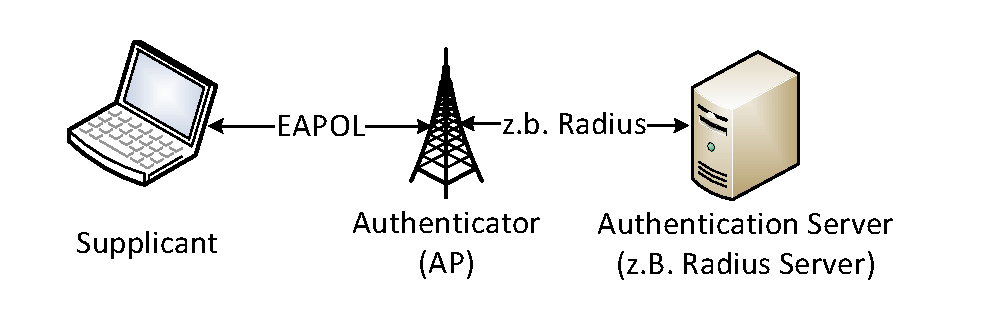
\includegraphics[scale=0.7]{figures/ap_radius}
\end{figure}
\end{frame}

\begin{frame}
\frametitle{Schlüsselhierarchie}
\end{frame}

\begin{frame}
\frametitle{4-Way-Handshake}
\begin{figure}
	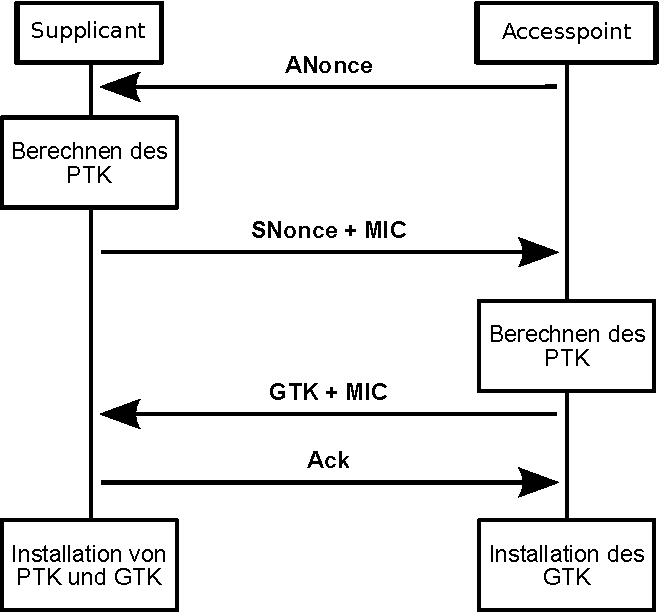
\includegraphics[width=0.5\linewidth]{figures/4-way-handshake.pdf}
	\caption{4-Way-Handshake nach \cite{ieee802.11}}
\end{figure}
\end{frame}

\begin{frame}
\frametitle{AES-CCMP}
\begin{itemize}
	\item AES-CCMP
\end{itemize}
\end{frame}

\begin{frame}
\frametitle{TKIP (Temporal Key Integrity Protocol)}
\begin{itemize}
	\item AES sollte in 802.11i integriert werden.
	\item AES Berechnungen aufwendig und erforderten neue Hardware
\end{itemize}
\begin{block}{Übergangslösung TKIP}
	\begin{itemize}
		\item Erweiterung von WEP
		\item RC4 weiterhin als Basis
		\item Dynamische statt statischer Schlüssel
		\item Größere IVs:
		\begin{itemize}
			\item 48 bit statt 24 bit
			\item Benutzt als TSC(TKIP Sequence Counter)
		\end{itemize}
		\item Michael (MIC) als verbesserte Intigritätsprüfung
	\end{itemize}
\end{block}
\end{frame}

\begin{frame}
\frametitle{Schwachstellen von TKIP}
\begin{itemize}
	\item Michael hat Schwachstellen (Brute-Force, DoS Angriffe, etc.)
	\item Wörterbuchangriff auf PBKDF2 langsam(4096 Runden HMAC-SHA1)
	\begin{itemize}
		\item Beschleunigung durch Rainbow Tables \cite{renderlab} (SSID + Passphrases)
		\item Berechnung in der Cloud \cite{cloudcracker}: 20 Minuten, 17\$, 300.000.000 Wörter
	\end{itemize}
\end{itemize}
\end{frame}


\begin{frame}
\frametitle{Hole 196}
\begin{itemize}
	\item Nur der AP darf Packete mit dem GTK verschlüsseln und an alle Clients senden
	\item Keine Überprüfung ob Packete wirklich vom AP kommen
    \item "Böser" Client nutzt den GTK um Packete an anderen Clients zu senden
	\item Kann nur von authorisierten Clienten ausgeführt werden
	\item Angriff im Standart dokumentiert.
\end{itemize}
\end{frame}

\section{Andere Attacken}
\subsection{WPS}

\begin{frame}
\frametitle{WPS (Wi-Fi Protected Setup)}
Drei Endnutzerfreundliche WLAN Konfigurationsmodi:
\begin{block}{Push-Button-Connect (“PBC”)}
Benutzer drückt physischen oder virtuellen Knopf.
\end{block}
\begin{block}{PIN - Internal Registrar}
Benutzer gibt mitgelieferten WPS Pin seines Endgerätes in Webmaske des AP ein.
\end{block}
\begin{block}{PIN - External Registrar}
Benutzer bekommt Pin vom Betreiber des APs mitgeteilt und gibt ihn in sein Endgerät ein.
\end{block}
\end{frame}


\begin{frame}
\frametitle{Angriff auf WPS, PIN - External Registrar \cite{wps_attack}}
\begin{itemize}
	\item PIN ist 8 Ziffern lang.
	\item Protokoll erlaubt es zu erkennen ob die ersten 4 Zeichen oder 4 Zeichen falsch waren.
	\item 8. Ziffern Checksumme der ersten 7 Ziffern.
	\item Zu testende Kombinationen: $10^4+10^3 = 11.000$
	\item WPS Standard schreibt kein Lockdown vor. Daher selten implementiert.
	\item Authentification benötigt im Schnitt 1,3 Sekunden.
\end{itemize}
\end{frame}

\subsection{User Tracking}
\begin{frame}
\frametitle{User Tracking}
\begin{itemize}
	\item Mülltonnen mit Werbebildschirmen und WLAN erfassten Fussgänger anhand ihrer Handies in London \cite{mulltonnen}
	\item Endgeräte auf der Suche nach versteckten SSIDs broadcasten den Namen der versteckten SSID
	\begin{itemize}
		\item Schlechte Implementationnen broadcasten auch den Namen der unversteckten SSIDs
	\end{itemize}
\end{itemize}
\end{frame}

\section{Häufige Absicherungsempfehlungen}
\begin{frame}
\frametitle{Häufige Absicherungsempfehlungen}
\begin{block}{MAC-Filter}
Kein Nennenswerter Sicherheitsgewinn, da MAC Adresse immer unverschlüsselt übertragen wird.
\end{block}
\begin{block}{SSID Verstecken}
AP broadcastet die SSID zwar nicht, aber sobald ein bekannter Teilnehmer sich anmeldet, wird die SSID unverschlüsselt übertragen.
\end{block} 
\begin{block}{Zufällige SSID}
Wörterbuchattacken gegen PBKDF2 nicht mehr so einfach.
\end{block}
\end{frame}

\section{Tools}
\begin{frame}
\frametitle{Tools}
\begin{block}{Aircrack-ng Suite (siehe \cite{aircrack})}
	\begin{description}
		\item[aircrack-ng] WEP, WPA, WPA2-PSK Key Cracker
		\item[aireplay-ng] Erzeugt WLAN Traffic
		\item[airdrop-ng] Regelbasiertes Deauth Tool
		\item[airodump-ng] Zeichnet WLAN Rohdaten auf
		\item[airdecap-ng] Entschlüsselt aufgezeichnete WEP, WPA, WPA2 Streams
		\item[...]
	\end{description}
\end{block}
\begin{block}{FakeAP (siehe \cite{fakeap})}
Simulieren falscher WLANs
\end{block}
\begin{block}{Kismet (siehe \cite{kismet})/NetStumbler (siehe \cite{netstumbler})}
WLANs aufspüren und kartografieren
\end{block}
\end{frame}

\section{References}
\begin{frame}[allowframebreaks]
\frametitle{References}
\bibliographystyle{IEEEtran}
% argument is your BibTeX string definitions and bibliography database(s)
\bibliography{references}
\end{frame}
\end{document}
